% %%%%%%%%%%%%%%%%%%%%%%%%%%%%%%%%%%%%%%%%%%%%%%%%%%%%%%%%%%%%%%%%%%%%%%%%%%%%%%%%
%
% example.tex :
% Based on example.tex by J. Dreissig (julian.dreissig@physik.de) for GSI Summer 
% Student Program 1999.
% Recycled for the Summer Student Program in 2007 and 2008.
% 
% This Latex2e file contains an example layout for your final report.
%
%   2007:
%   Maciek Sobczak, macieksobczak@wp.pl
%   Friedemann Zenke, fzenke@gmail.com
%
%   2008:
%   04herbst@edu.uni-graz.at
%
% %%%%%%%%%%%%%%%%%%%%%%%%%%%%%%%%%%%%%%%%%%%%%%%%%%%%%%%%%%%%%%%%%%%%%%%%%%%%%%%%
% DO NOT EDIT!
% BEGIN Header
\documentclass[twocolumn,gsifonts,twoside]{gsipaper}
\usepackage{a4wide,gsiindex,helvet}
\usepackage[english]{babel}
\usepackage{amsmath,amsfonts,amssymb,verbatim,float}
\usepackage[pdftex]{graphicx} % Graphic files: pdf or jpg

\begin{document}
% END Header

% Edit below this line
% %%%%%%%%%%%%%%%%%%%%%%%%%%%%%%%%%%%%%%%%%%%%%%%%%%%%%%%%%%%%%%%%%%%%%%%%%%%%%%%%


% -= NOTA BENE =-
% Replace the title, abstract, authors, and addresses within the curly brackets
% with your own title, authors, and  addresses. You may have as many authors and
% addresses as you need.  The control sequences of author and addresses can be
% repeated as often as necessary. Footnotes in titles, adresses and the abstract
% need a special procedure and are described below.

\title{Quality Assurance of silicon sensors for CBM-STS}

\abstract{This report introduces CBM-STS detector and the Quality Test Center(QTC)
	in GSI. It also details the hardware and setup for quality assurance as well as
	the QA procedures, which includes optical and electrical inspection. The database
	framework for CBM-STS QA has been implemented using	the FairDB SQL Interface, 
	and QA data schemes would be shown in this paper. In addition, several diagrams
	extracting from measurement data are given.
	}

\shortauthor{Wu, Yitao}
\shorttitle{CBM-STS QA}

\author{Yitao Wu}            % first author
\address{University of Science and Technology of China, torrence@mail.ustc.edu.cn}

%\author{next author}                  % if you have more than one author,
%\address{next address}                % use these lines for the next one.

\maketitle
%\thispagestyle{empty}

% -= NOTA BENE =-
% Start your text with the following command. 

\section{Introduction}
The Compressed Baryonic Matter (CBM) experiment will carry out
systematic research on the properties of nuclear matter under extreme conditions,
in particular, at highest net baryon densities. These conditions will
be met by colliding beams of heavy ions on targets in the energy range from
2 to 14, eventually 45 GeV/nucleon, as they will be provided with highest
intensities by the heavy-ion synchrotron SIS-100, and in a future stage
by the SIS-300 machine of the Facility for Anti-proton and Ion Research
(FAIR) at GSI, Darmstadt, Germany.

\subsection{Silicon Tracking System}
Objective, Requirements, Design, Principle, Geometry, Readout, DAQ

The Silicon Tracking System (STS) is the central detector fo the CBM
experiment at FAIR. Its task is the standalone trajectory reconstruction
of the high multiplicities of charged particles originating from high-rate
beam-target interactions. The silicon microstrip detectors must be
radiation hard and are read out by a fast self triggering front-end
electronics.

\subsection{Quality Test Center}
Motivation program of QA. Task and condition in QTC

Due to a large-scale sensor production, the effective QA of sensors can be
achieved by a collective effort among the Quality Test Centers. [Figure]
indicates the variety of quality assurance tests and the corresponding QTC
in charge. The overall QA program can be represented as a combination of
tests performed on sensor and strip level.

\paragraph{Optical inspection} is intended to identify any kinds of surface
defects. This test will be performed on 100\% of the sensors at the EKU
test center. Sensors with identified defects will undergo further electrical
tests.

\paragraph{Bulk electrical tests} are performed to determine the overall
sensor behavior at the operational conditions. Current-voltage (I-V) and
capacitance-voltage (C-V) tests are conducted after optical inspection. The
I-V tests determines the leakage current of a sensor while the C-V tests
determines the full depletion voltage of a sensor.

\paragraph{Long-term stability tests} will be performed on a fraction of the
sensors. The leakage current of the sensors will be monitored for a time period
of 48-72 hours in order to evaluate their stability.

\paragraph{Microscopic electrical tests} focus on determination of various sensor
parameters and their correspondence with specifications, mainly coupling
capacitance $C_{c}$, interstrip capacitance $C_{is}$, interstrip resistance
$R_{is}$, and bias resistance $R_{bias}$.

\paragraph{Strip diagnostic tests} aim to identify strip defects originating
from the complex fabrication process that cannot be identified by the optical
inspection. These defects comprise mainly ohmic contacts or short circuits
between the strip implant and the readout strip (so-called ``pinholes''), short
circuits between two or more readout strips, and strips exhibiting high leakage
current.

\section{Hardware and Setup}
\subsection{Testing conditions}
\subsection{Storage conditions}
\subsection{Equipment and testing tools/devices}

\section{Quality Assurance in GSI}
\subsection{Optical Inspection}
\subsection{Electrical Inspection}

\section{QA Database}
\subsection{FairDB}
\subsection{Some Results}

\section{Summary}

\section{Guidelines}
\subsection{Writing your report}\label{ywu:writing}

If you unpacked the archive correctly, you should have a directory
named \textsf{report} containing the following files\footnote{You
  probably obtained these files from the web. And by the way this is
  how you make a footnote.} 

\noindent {\sf  gsipaper.cls}   ---  the class file that provides the  higher
                     level \LaTeX\ commands for the reports. Don't change
                     these parameters.

\noindent {\sf  gsiindex.sty}   ---  a style file that also provides something,
                               but you should not bother.


\noindent {\sf  example.tex}  ---  the main text - this is what you
are reading now. 

\noindent {\sf  fig.pdf}  ---  a little plot in in the pdf format.

\noindent {\sf  SummerBanner.jpg}  ---  a graphic in jpg format.

You can delete my sample text and replace it with your own
contribution to the volume, however we recommend keeping a copy of the
initial version of the file for reference.  We work with
\verb|pdflatex|, which implies that the format of figures is either
\verb|pdf| or \verb|jpg|.  If you use an editor adapted to deal with
\LaTeX , such as \verb|kile| or \verb|emacs| under \verb|LINUX| or the
\verb|LEd| (Latex editor) together with the package
\verb| "MiKTeX 2.8"| under Microsoft, care that the processing is done
as \verb|pdflatex|; the \verb|TeXShop| editor under MacOS
automatically works with \verb|pdflatex|.  On the commandline level,
the command for latexing is \verb|pdflatex template.tex|, do this
twice to sort out the cross-referencing.

These files should work with standard pdf\LaTeX. Page numbers are
included at the bottom of the page for your guidance. Do not worry
about the final pagination of the volume which will be done after you
have submitted the paper.

label
\subsection{Headings and Text}

Please preserve the style of the headings, text fonts and line spacing
to provide a uniform style for the reports volume.  In a two column
format there may arise difficulties when finding suitable line and
page breaks. We would strongly recommend that you leave such problems
until preparing the final draft and after you have checked the placing
of the two-column wide tables etc.


\subsection{Equations}

You can use inline equations, like $1 = 2 \pm 1$, but you should make
sure that equations should be confined to one column wherever
possible. Use the {\it equation} environment to display equations that
you would like to reference to
\begin{equation}
  a^2 + b^2 = c^2
  \label{ywu:eqn:pythagoras}
\end{equation}
like this (see very important Eqn.\,\ref{ywu:eqn:pythagoras}) or use
the {\it align} environment to split equations into several lines,
and/or to align several equations with the \& tabulator, {\em cf}.
Eqs.\,(\ref{ywu:eq:murnf}\,-\,\ref{ywu:eq:potential}).  The second
equation contains also some formatting hints concerning spacing using
$\sim$ or $\backslash$, or $\backslash$!  etc.  and the insertion of
text into formulae.  If it's essential to have a two-column wide
equation then use the method of
Eqs.\,(\ref{ywu:eq:murnf}\,-\,\ref{ywu:eq:potential}).

\begin{figure*}[tb] % {figure*} = page-wide figure; 
  % placement directive tb = preferred "top" else "bottom"
  % 
  \begin{align}       % aligning equations with tabulator &
    U &= D(\delta_1 , \delta_2 , \delta_3 , \delta_4)
    R_{12}(a,\delta_5)R_{13}(b,\delta_6)R_{14}(c,\delta_7)R_{23}(d,\delta_8)
    R_{24}(e,\delta_9)R_{34}(f,\delta_{10})
    \label{ywu:eq:murnf}
    \\
    V(\vec{r}\,)&=\int_{-\infty}^{\vec{r}}\vec{F}(\vec{r}\,')\,{\rm d}\vec{r}\,'
    ~~~\mbox{for}~~~ \vec{r}\in {\rm I\!R}^3
    ~~~\mbox{(potential energy)}
    \label{ywu:eq:potential}
  \end{align}
\end{figure*}


For problems of placement of a wide equation, see  Section
\ref{ywu:limits} below. 


\subsection{Tables}

The tables are designed to have a uniform style throughout the reports
volume. It doesn't matter how you choose to place the inner lines of
the table, but we would prefer the border lines to be of the style
shown in Tables \ref{ywu:tab:smtab} and \ref{ywu:tab:exp}. For either a
single or a double column table, the top and bottom horizontal lines
should be single (using {\it $\backslash$hline}), and there should be
single vertical lines on the perimeter, (using {\it
  $\backslash$begin\{tabular\}\{$|...|$\}}) as in Tables
\ref{ywu:tab:smtab} and \ref{ywu:tab:exp}.  For the inner lines of the
table, it looks better if they are kept to a minimum.

The use of single column-wide tables is recommended wherever possible. For the
page wide tables, use the environment given in the example of
Table\,\ref{ywu:tab:exp}. Do \textbf{not} change the latex commands from
{\it $\backslash$begin\{table*\}} to
{\it $\backslash$begin\{tabular\}}, or from
{\it $\backslash$end\{tabular\}} to
{\it $\backslash$end\{table*\}},
apart from inserting your own caption and table label. The captions
for tables and figure should be placed at the bottom.

\begin{table}[t]   % placement directive: t = top of column
  \center
  \begin{tabular}{|c|c|c|c|}
    \hline
    \raisebox{0pt}[12pt][6pt]{Title} &
    \raisebox{0pt}[12pt][6pt]{$\epsilon^{\prime}$} &
    \raisebox{0pt}[12pt][6pt]{$\lambda$} &
    \raisebox{0pt}[12pt][6pt]{$\gamma$} \\
    \hline
    \raisebox{0pt}[12pt][6pt]{12} &
    \raisebox{0pt}[12pt][6pt]{34} &
    \raisebox{0pt}[12pt][6pt]{56} &
    \raisebox{0pt}[12pt][6pt]{78} \\

    \cline{1-2}
    \multicolumn{2}{|c|}{\raisebox{0pt}[12pt][6pt]{and even more importantly}} 
    & &\\\cline{1-2}
    \raisebox{0pt}[12pt][6pt]{6.8977} &
    \raisebox{0pt}[12pt][6pt]{8.9087} &
    \raisebox{0pt}[12pt][6pt]{\textbf{42}} &
    \raisebox{0pt}[12pt][6pt]{4.2928} \\\hline
  \end{tabular}
  \caption{Small Table with some fancy input}\label{ywu:tab:smtab}
\end{table}


\begin{figure}[b]  % placement directive: b = bottom of column
  \center
  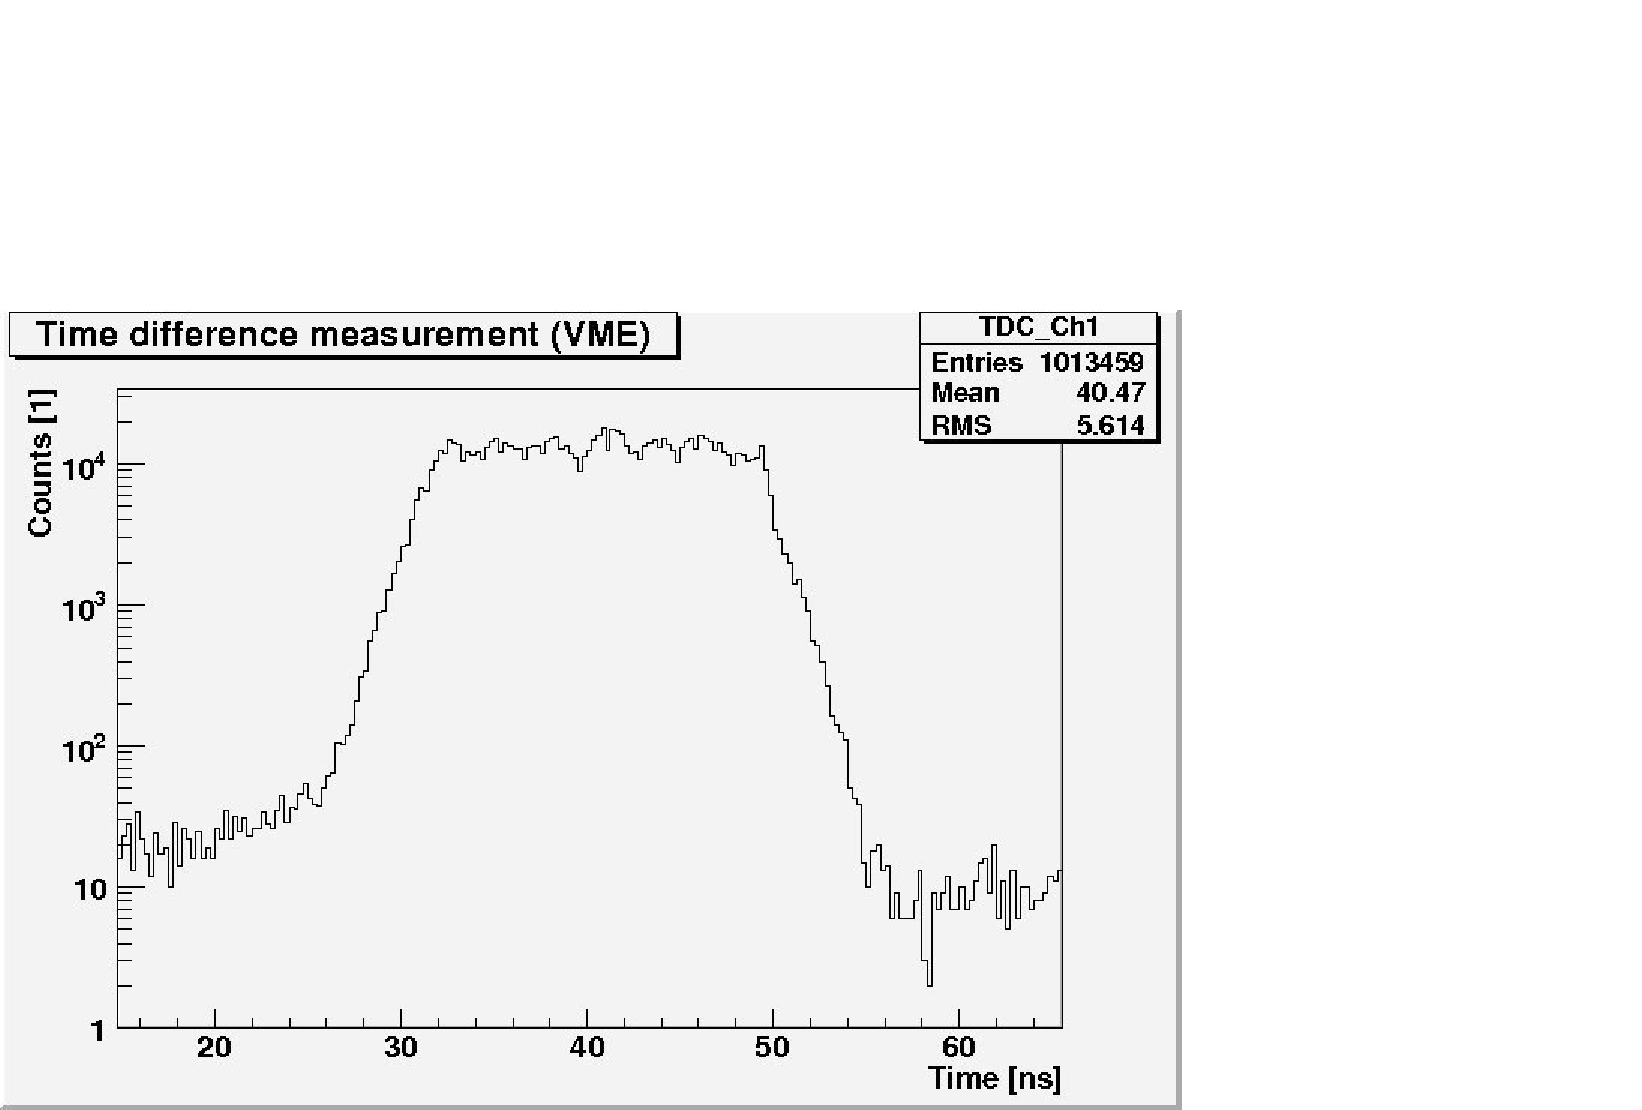
\includegraphics[width=0.45\textwidth]{ywu-pic}
  \caption{Caption for the figure will come here.}
  \label{ywu:fig:radk}
\end{figure}

\subsection{Figures}

The same arguments as given above also apply for figures, i.e. it is
preferable to have figures that fit into one column of the text. If
this is not possible, then use the full page-width 
commands {\it $\backslash$begin\{figure*\}} and {\it
  $\backslash$end\{figure*\}}. The {\it $\backslash$includegraphics}
command can take optional arguments such as width or height of the
graphics, as can be seen in the examples given in this document.
\LaTeX\ will scale the figure based on the width provided and adjust
the height accordingly. You can use any form of the units of
measurement described in the \LaTeX\ Book.

Preferred graphic formats are \textit{pdf}- or \textit{jpg}. You will
find this format amongst other output formats of most graphics
software. The \textit{eps} format is allowed!  DO NOT - I repeat - DO
NOT use the Unix command \verb|convert| unless you really know what
you are doing!



\begin{table*}[t]
  \begin{tabular}{|c|c|c|p{187pt}|}
    \hline
    \raisebox{0pt}[16pt][6pt]{Meson} &
    $\Gamma(\pi^+\pi^-)\; s^{-1}$ &
    $\Gamma(\pi^+\pi^-\gamma)\; s^{-1}$ &{} \\[3pt]
    \hline
    \hline
    \raisebox{0pt}[16pt][6pt]{$K^0_S$}    & $0.769 \times 10^{10}$ &
    $5.46 \times 10^7$ &
    No DE observed, not even (IB)-E1
    interference, despite large statistics, for $E^{\ast}_{\gamma} >
    20$MeV.\\[6pt]
    \hline

    $K^0_L$ &
    $3.93 \times 10^4$ &

    $ (\rm{DE} = 0.62 \times 10^3)$ &
    DE prominent, exceeding IB over the  range of measurement $20 <
    E^{\ast}_{\gamma} < 160$MeV.\\[6pt]
    \hline
  \end{tabular}
  \caption{Nonsense Data. Note the difference between with(out)
    \textit{raisebox} attribute in the code \label{ywu:tab:exp}} 
\end{table*}


\subsection{Limitations on the Placement of Equations, Tables
and Figures}\label{ywu:limits}

Figures and tables are so-called float objects that the \LaTeX
processor tries locate into some available space in the columns or at
the page according to the directives given in square brackets, like
[tb]. In order to have these float objects properly placed it may be
necessary to shift the figure of tables declaration to appropriate
places in the \LaTeX source file. Thus, in the final stages of
preparing the document, try to declare the two-column wide figures,
tables or equations at a point in {\it example.tex} that is prior to
the top of the column of text where you would like the item to
appear.\footnote{By `declaring' I refer to placing the chunk of
  material describing the table or whatever at a particular point in
  the tex file.} 
\begin{figure}[htb] % directives: here, top, bottom
  \unitlength0.01\textwidth
  \begin{picture}(40,8) % (width,height) in \unitlength
    \put(0,0){
\includegraphics[width=0.45\textwidth]{ywu-SummerBanner}}
    \put(2,6){\sf\large HGS-HIRe Summer Student}
    \put(2,1){\sf\large Program at GSI}
  \end{picture}
  \caption{Summer banner in picture environment}
  \label{ywu:fig:banner}
\end{figure}
If you want to place an oversized object, as shown above in
Fig.\,\ref{ywu:fig:banner} for our logo reaching out of the standard
text area, wrap the object by the {\it picture} environment of proper
size. You can add further picture elements like text, etc.

For {\it figure} environments try to use {\it
  $\backslash$begin\{figure\}$[$htb$]$} (which is the default) where
ever you can. Only very large figures and tables should be placed on a
page by themselves. One can use the instruction {\it
  $\backslash$begin\{figure*\}$[$p$]$} or {\it
  $\backslash$begin\{table*\}$[$p$]$} to position these, and they will
appear on a separate page devoted to figures and tables. Again, we
would recommend making any necessary adjustments to the layout of the
figures and tables only in the final draft. It is also simplest to
sort out line and page breaks in the last stages.


\subsection{Footnotes, the Bibliography, and Acknowledgments} \label{ywu:foot}

Acknowledgments to tutors etc. may be placed in a separate section at
the end of the text, before the bibliography.  This should not be
numbered so use {\it $\backslash$section*\{Acknowledgements\}}.

Footnotes are denoted by a letter superscript in the text, and
references are denoted by a number in square brackets. We have used
{\it $\backslash$bibitem} to produce the bibliography. Citations in
the text use the labels defined in the bibitem declaration, for
example, the first paper by Jarlskog\cite{ywu:ja} is cited using the
command {\it $\backslash$cite\{ywu:ja\}}.


\subsection{Your own packages}

If you like to use other packages than the already provided ones ({\it
  amsmath, amsfonts, verbatim, graphicx, float}) please use an extra
{\it $\backslash$usepackage\{...\}} line, since we will cut off the
marked lines at the top of the document as indicated in the comments.
If you use non-standard packages please include them in your tarfile.

\section{Happy \LaTeX{}ing and howto submit your manuscript}

Once you finished writing your report, please print it out and check
it once more for misspellings etc. If you have already done it, do it
again. We won't be able to find typos in your formulas. So check them
carefully! Also please check your bibliography items. See whether the
figures and tables appear in the positions you would like to have
them, otherwise move them.  If you think, everything that could be
done is done, which means that you triple and quadruple checked
everything, please save your \TeX file as \verb|report_yourname.tex|
and `zip' your files (including the images and whatsoever) into one
archive \verb|yourname.zip| (e.g. under LINUX: 
\verb|zip -r yourname.zip yourdirectory|). Then send the
resulting file to the Summer Student in charge of compiling the book.
Please refrain from sending your file twice or more to avoid
unecessary confusion on his side.


\section*{Acknowledgments}

Olga, Anton;
Muksym?, Hanna, Adrian, ...;
Summer students;
Joern, Gabi, orgnizers, lecturers, GSI

\begin{thebibliography}{99}

\bibitem{ywu:ja}
C Jarlskog in {\it CP Violation}, ed. C Jarlskog
(World Scientific, Singapore, 1988).

\bibitem{ywu:ma}
L. Maiani, {\it Phys. Lett.} B {\bf 62}, 183 (1976).

\bibitem{ywu:bu}
J.D. Bjorken and I. Dunietz, {\it Phys. Rev.} D {\bf 36}, 2109 (1987).

\end{thebibliography}

% %%%%%%%%%%%%%%%%%%%%%%%%%%%%%%%%%%%%%%%%%%%%%%%%%%%%%%%%%%%%%%%%%%%%%%%%%%%%%%%%
% Do NOT edit below this line
% %%%%%%%%%%%%%%%%%%%%%%%%%%%%%%%%%%%%%%%%%%%%%%%%%%%%%%%%%%%%%%%%%%%%%%%%%%%%%%%%

\end{document}

% %%%%%%%%%%%%% END OF example.tex %%%%%%%%%%%%%%%%%%%%%%%%%%%%%%%%%%%%%%%%%%%%%%%